\section{Transistor models}\label{sec:models}
\subsection{Targets, preprocessing and metrics}
The four terminal currents span about ten decades, change sign, and part of the data is numerical noise (Section~2). Each current $I$ is therefore
modelled through the signed-logarithmic target
\[
  y=\frac{\operatorname{asinh}(I/I_0)}{\ln 10},\qquad I_0=10^{-15}\,\mathrm{A},
\]
which behaves like $\operatorname{sign}(I)\log_{10}(2|I|/I_0)$ for $|I|\gg I_0$, is linear (and exactly zero for $I=0$) below $I_0$, and thus treats
sign changes, zeros and ten decades of dynamic range in one continuous variable. Targets are standardised per column. Inputs are the
physically motivated features $\log_{10}W$, $1000/T[\mathrm{K}]$, $V_{DD}$, $V_d$, $V_s$, $V_{ds}$, $V_{gs}$, $V_{gd}$, $V_{bs}$, $V_{bd}$, $|\text{vth0}|$,
toxe, $\log_{10}$ndep, u0, xj, standardised.

Each dataset is split randomly into $70\%/15\%/15\%$ (7{,}000/1{,}500/1{,}500) training/validation/test sets with a fixed seed (stored in \texttt{data/splits}).
All hyper-parameters and the model choice use the validation set only; the test set is evaluated once, for the chosen model.

\paragraph{Metrics.} The relative error $|I_{ML}-I_{SPICE}|/|I_{SPICE}|$ is computed on the \emph{resolved} samples ($|I_{SPICE}|>I_0$), because below $I_0$ the reference
values are noise of the BSIM4 evaluation and cannot be predicted (Section~2). Currents with fewer than 5\,\% resolved samples (the gate current of the OFF devices) are
not scored. $R^2$ is computed on the signed-log target. The tables report the average over the scored currents; per-current values are in \texttt{results/models/}.

\subsection{Model families}
Four model types were trained for each case (as required by the course-group clarification):
\begin{enumerate}[nosep]
\item \textbf{MLP}: fully connected network, 3 hidden layers of 96 or 128 tanh units, float64, trained with Adam (mini-batch 256, cosine learning-rate decay from $3\cdot10^{-3}$,
      1200 epochs) followed by full-batch L-BFGS polishing; the loss weights the pure-noise currents by 0.02, and the epoch with the best (weighted) validation loss is kept.
\item \textbf{Gradient-boosted trees} (LightGBM): one regressor per current, 31 or 127 leaves, learning rate 0.05, early stopping on validation.
\item \textbf{Kernel ridge regression} with RBF kernel ($\gamma\in\{0.01,0.03,0.1\}$, $\alpha\in\{10^{-5},10^{-3}\}$).
\item \textbf{Polynomial ridge regression} (degree 3 or 4, $\alpha\in\{10^{-3},10^{-1},10\}$).
\end{enumerate}
A first round used scikit-learn's L-BFGS MLP; it was under-trained and weighted the noise currents like all others, which hurt the OFF cases
(results kept in \texttt{results/models/round1\_sklearn\_mlp/}). The reported MLP is the improved PyTorch version.

\subsection{Comparison and choice}
\begin{table}[H]
\centering
{\small
\begin{tabular}{llrrrl}
\toprule
case & model & R2 (signed-log) & median err & 95th pct err & best hyper-parameters \\
\midrule
nmos\_off & kernel\_ridge & 0.9316 & 42.69\% & 161.28\% & gamma: 0.01, alpha: 0.001 \\
nmos\_off & lightgbm & 0.9794 & 8.78\% & 63.18\% & num\_leaves: 31 \\
nmos\_off & mlp & 0.9951 & 1.69\% & 14.82\% & hidden: (96, 96, 96), epochs: 1200, activation: tanh, polish\_rounds: 6, polish\_iter: 300, threads: 2 \\
nmos\_off & poly\_ridge & 0.9302 & 41.67\% & 232.97\% & degree: 4, alpha: 0.1 \\
nmos\_on & kernel\_ridge & 0.9281 & 69.44\% & 5359.93\% & gamma: 0.01, alpha: 0.001 \\
nmos\_on & lightgbm & 0.9976 & 12.63\% & 61.72\% & num\_leaves: 31 \\
nmos\_on & mlp & 0.9963 & 4.30\% & 22.29\% & hidden: (128, 128, 128), epochs: 1200, activation: tanh, polish\_rounds: 6, polish\_iter: 300, threads: 2 \\
nmos\_on & poly\_ridge & 0.9068 & 71.43\% & 30690.41\% & degree: 4, alpha: 10.0 \\
pmos\_off & kernel\_ridge & 0.9383 & 35.69\% & 151.66\% & gamma: 0.03, alpha: 0.001 \\
pmos\_off & lightgbm & 0.9785 & 8.56\% & 65.10\% & num\_leaves: 31 \\
pmos\_off & mlp & 0.995 & 4.29\% & 24.75\% & hidden: (128, 128, 128), epochs: 1200, activation: tanh, polish\_rounds: 6, polish\_iter: 300, threads: 2 \\
pmos\_off & poly\_ridge & 0.9287 & 40.06\% & 187.49\% & degree: 4, alpha: 0.001 \\
pmos\_on & kernel\_ridge & 0.9327 & 68.42\% & 4639.72\% & gamma: 0.01, alpha: 0.001 \\
pmos\_on & lightgbm & 0.9968 & 13.15\% & 65.96\% & num\_leaves: 31 \\
pmos\_on & mlp & 0.9995 & 2.04\% & 12.16\% & hidden: (96, 96, 96), epochs: 1200, activation: tanh, polish\_rounds: 6, polish\_iter: 300, threads: 2 \\
pmos\_on & poly\_ridge & 0.9137 & 70.11\% & 27706.76\% & degree: 4, alpha: 10.0 \\
\bottomrule
\end{tabular}
}
\caption{Model comparison on the \emph{validation} set (4 model types $\times$ 4 cases). Errors are relative errors on currents above the noise floor, averaged over the scored currents.}
\label{tab:comparison}
\end{table}


The MLP is the most accurate model in all four cases, by a large margin over the other three families. Kernel ridge and polynomial regression, which assume
a smooth global dependence, cannot follow the exponential and threshold-like behaviour (sub-threshold and tunnelling currents) over ten decades;
gradient boosting is robust but piecewise-constant and cannot reach the precision of the MLP. The MLP was therefore selected for all four cases.

\subsection{Chosen models on the test set}
\begin{table}[H]
\centering
{\small
\begin{tabular}{lllrrr}
\toprule
case & model & currents scored & median err & 95th pct err & R2 (signed-log) \\
\midrule
nmos\_on & mlp & id,ig,is,ib & 4.05\% & 22.72\% & 0.998 \\
nmos\_off & mlp & id,is,ib & 1.62\% & 20.18\% & 0.9919 \\
pmos\_on & mlp & id,ig,is,ib & 1.91\% & 11.32\% & 0.9992 \\
pmos\_off & mlp & id,is,ib & 4.23\% & 22.66\% & 0.9979 \\
\bottomrule
\end{tabular}
}
\caption{Chosen models, test-set summary (macro-average over the scored currents).}
\label{tab:chosen_macro}
\end{table}


\begin{table}[H]
\centering
{\small
\begin{tabular}{lllrrrrr}
\toprule
case & model & current & frac. resolved & R2 (signed-log) & median err & 95th pct err & bias \\
\midrule
nmos\_on & mlp & id & 98.87\% & 0.9964 & 5.59\% & 32.30\% & 0.30\% \\
nmos\_on & mlp & ig & 82.20\% & 0.9994 & 2.79\% & 14.85\% & 0.00\% \\
nmos\_on & mlp & is & 98.87\% & 0.9965 & 5.16\% & 33.47\% & 0.31\% \\
nmos\_on & mlp & ib & 75.93\% & 0.9997 & 2.66\% & 10.27\% & -0.07\% \\
nmos\_off & mlp & id & 53.33\% & 0.9918 & 1.85\% & 20.71\% & 1.02\% \\
nmos\_off & mlp & ig & 0.00\% & 0.9946 & -- & -- & -- \\
nmos\_off & mlp & is & 53.80\% & 0.9841 & 1.94\% & 33.09\% & 0.16\% \\
nmos\_off & mlp & ib & 43.47\% & 0.9998 & 1.09\% & 6.74\% & -0.24\% \\
pmos\_on & mlp & id & 98.87\% & 0.9985 & 2.63\% & 17.00\% & -0.82\% \\
pmos\_on & mlp & ig & 85.20\% & 1 & 1.11\% & 5.23\% & -0.03\% \\
pmos\_on & mlp & is & 98.87\% & 0.9985 & 2.59\% & 16.72\% & -0.75\% \\
pmos\_on & mlp & ib & 75.13\% & 0.9998 & 1.32\% & 6.34\% & 0.11\% \\
pmos\_off & mlp & id & 54.13\% & 0.9974 & 4.74\% & 29.65\% & -1.17\% \\
pmos\_off & mlp & ig & 0.00\% & -0.1168 & -- & -- & -- \\
pmos\_off & mlp & is & 54.60\% & 0.9971 & 4.63\% & 25.66\% & -0.40\% \\
pmos\_off & mlp & ib & 44.33\% & 0.9993 & 3.31\% & 12.65\% & -0.15\% \\
\bottomrule
\end{tabular}
}
\caption{Chosen models on the \emph{test} set, per terminal current (errors on samples with $|I|>10^{-15}$\,A).}
\label{tab:chosen}
\end{table}


\begin{figure}[H]\centering
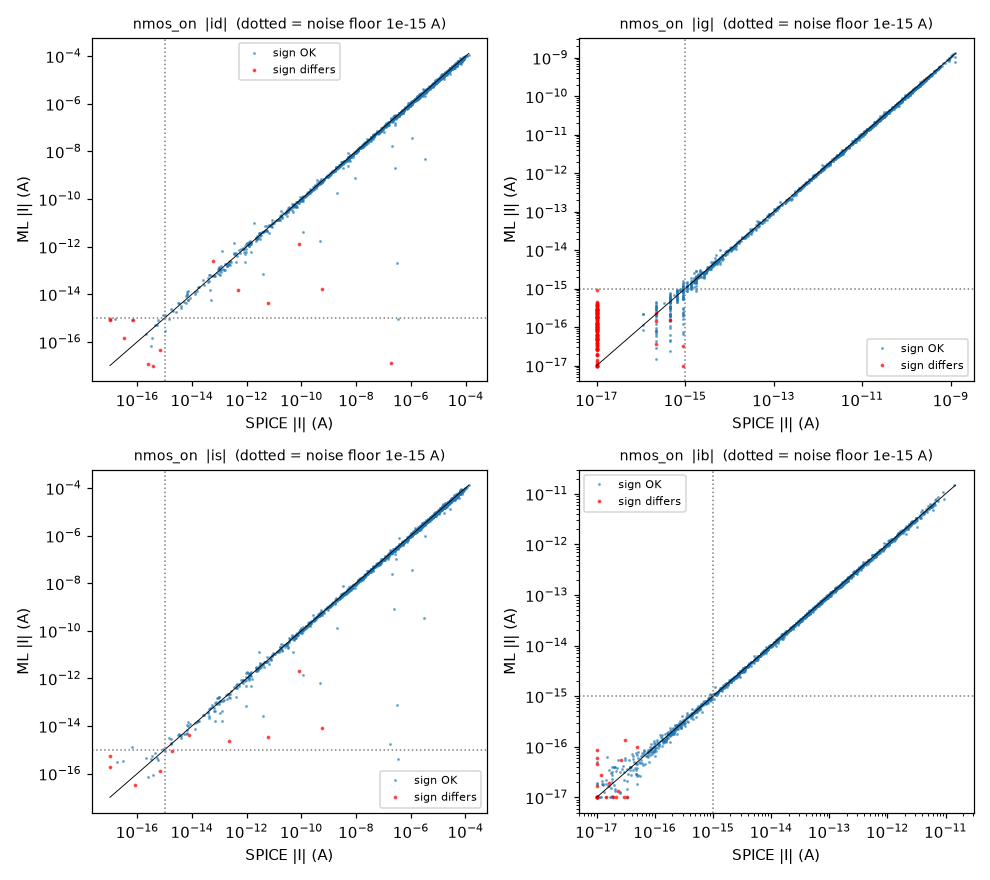
\includegraphics[width=.49\textwidth]{pred_vs_spice_nmos_on.png}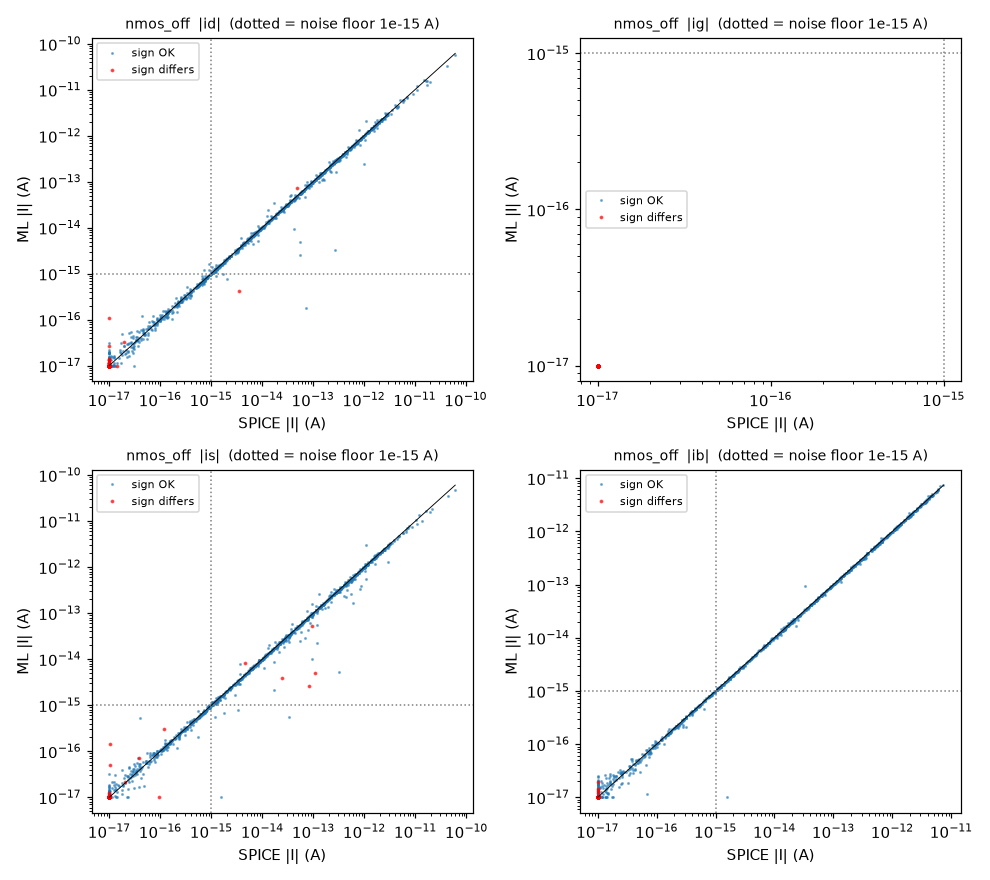
\includegraphics[width=.49\textwidth]{pred_vs_spice_nmos_off.png}\\
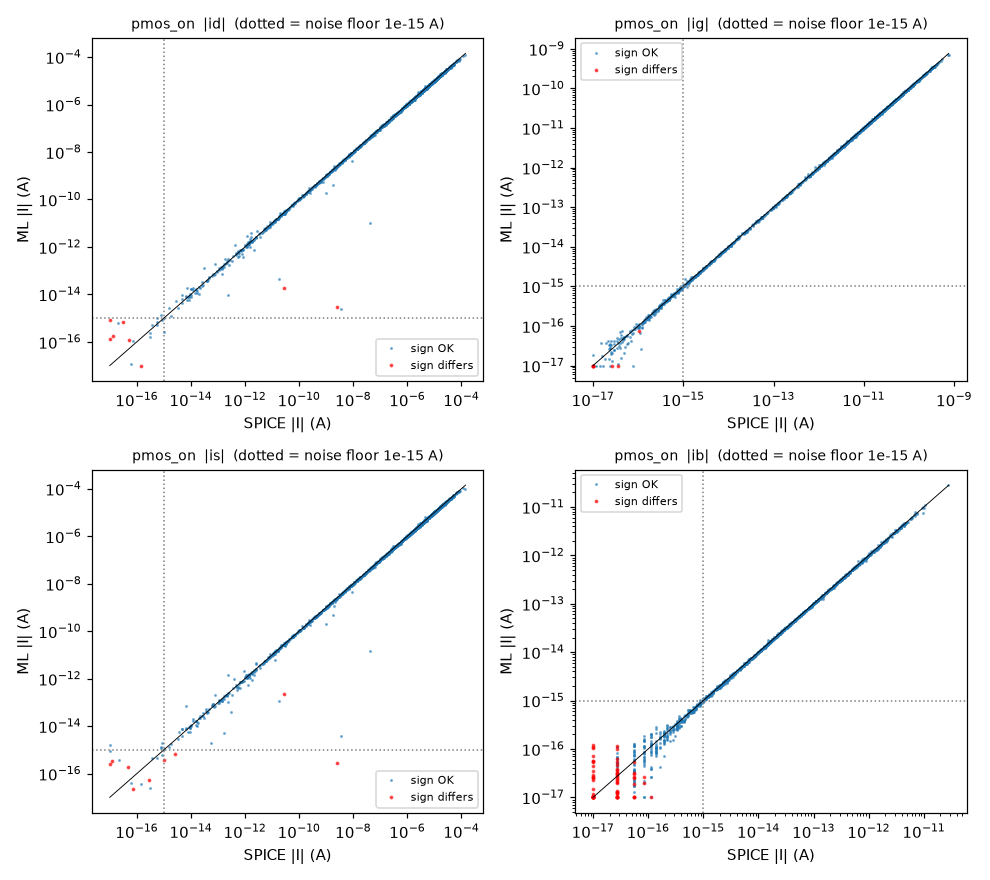
\includegraphics[width=.49\textwidth]{pred_vs_spice_pmos_on.png}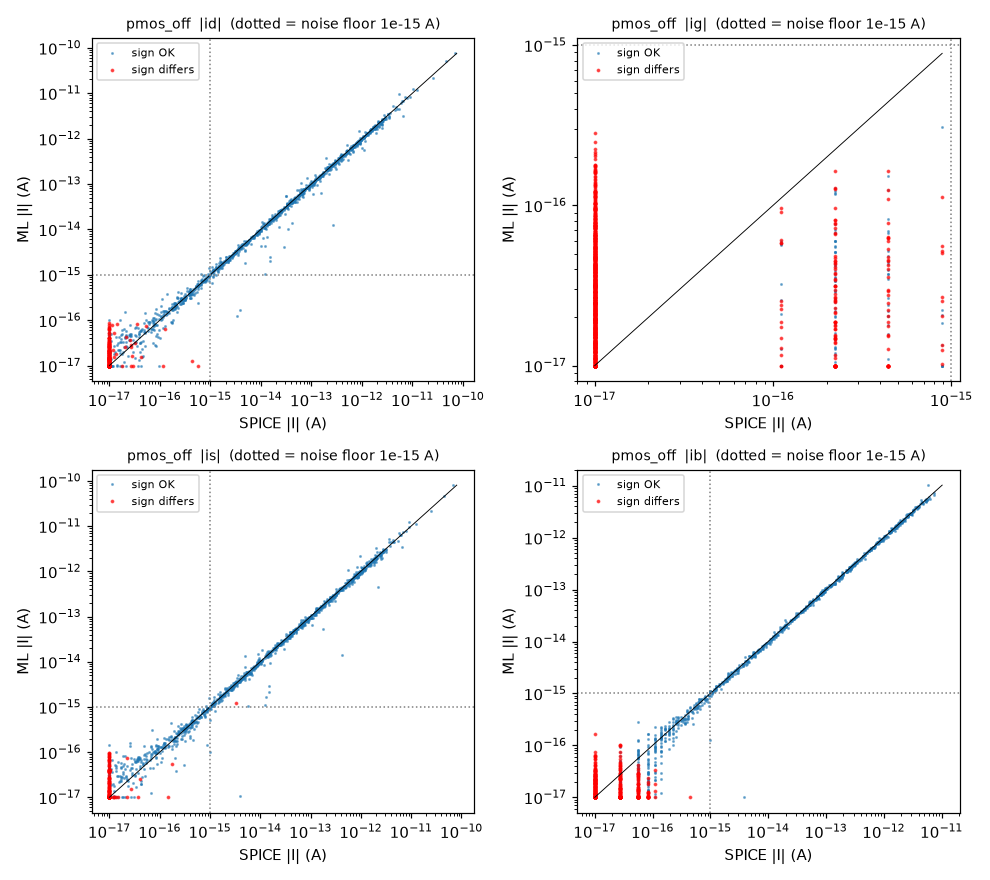
\includegraphics[width=.49\textwidth]{pred_vs_spice_pmos_off.png}
\caption{Predicted versus SPICE current (absolute value, log axes) on the test set for the four chosen models. The dotted lines mark the noise floor $10^{-15}$\,A.}
\end{figure}
The median error is $1.6$--$4.2\%$ and the 95th percentile $11$--$23\%$ (test set, resolved currents), with biases below 1.2\,\%. The NMOS OFF model is the most accurate and the
PMOS OFF model the least; for the ON models the relative error is largest for the smallest channel currents (small $V_{ds}$ or little gate overdrive), where the current changes sign.

\subsection{Learning curve}
\begin{table}[H]
\centering
{\small
\begin{tabular}{lrrr}
\toprule
case & train samples & val median err & val 95th pct err \\
\midrule
nmos\_on & 500 & 23.72\% & 141.57\% \\
nmos\_on & 1000 & 15.17\% & 70.17\% \\
nmos\_on & 2000 & 7.62\% & 53.72\% \\
nmos\_on & 4000 & 5.75\% & 29.50\% \\
nmos\_on & 7000 & 4.30\% & 22.29\% \\
nmos\_off & 500 & 26.91\% & 122.77\% \\
nmos\_off & 1000 & 11.40\% & 76.03\% \\
nmos\_off & 2000 & 4.80\% & 41.52\% \\
nmos\_off & 4000 & 3.08\% & 25.48\% \\
nmos\_off & 7000 & 1.69\% & 14.82\% \\
pmos\_on & 500 & 22.52\% & 118.21\% \\
pmos\_on & 1000 & 9.79\% & 67.54\% \\
pmos\_on & 2000 & 5.80\% & 40.47\% \\
pmos\_on & 4000 & 3.02\% & 17.90\% \\
pmos\_on & 7000 & 2.04\% & 12.16\% \\
pmos\_off & 500 & 37.93\% & 133.35\% \\
pmos\_off & 1000 & 19.70\% & 79.02\% \\
pmos\_off & 2000 & 11.82\% & 56.38\% \\
pmos\_off & 4000 & 5.31\% & 32.97\% \\
pmos\_off & 7000 & 4.29\% & 24.75\% \\
\bottomrule
\end{tabular}
}
\caption{Validation error of the chosen model versus training-set size.}
\label{tab:lc}
\end{table}


\begin{figure}[H]\centering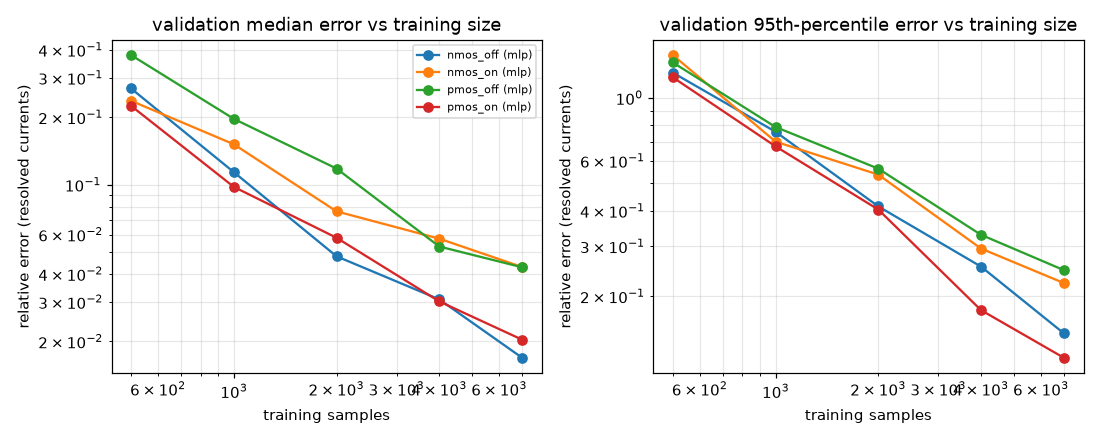
\includegraphics[width=\textwidth]{learning_curve.png}\caption{Validation error of the chosen model versus training-set size.}\end{figure}
The error has \emph{not} saturated at 7{,}000 training samples: each doubling of the data reduces the median error by roughly a third to a half. The assignment allows the sample
count to be increased; Section~\ref{sec:enlarged} reports the result of doing so.
\subsection{Extension: enlarged training set (assumption A4)}\label{sec:enlarged}
Because the learning curves had not saturated and the assignment allows the number of samples to be increased, $30{,}000$ additional samples per case were drawn from the same distributions
(independent random stream) and used as extra \emph{training} data; the validation and test sets are the original ones, so all numbers are directly comparable. The comparison of the four model types
above is unchanged (it uses the specified $10{,}000$-row dataset); only the winning type, the MLP, was refit on $37{,}000$ training rows (1500 epochs; a first attempt with 500 epochs was under-trained and made the NMOS ON model worse).
\begin{table}[H]
\centering
{\small
\begin{tabular}{lrrrrr}
\toprule
case & train rows (enlarged) & median err (10k) & median err (enlarged) & 95th pct (10k) & 95th pct (enlarged) \\
\midrule
nmos\_on & 37000 & 4.05\% & 7.15\% & 22.72\% & 23.63\% \\
nmos\_off & 37000 & 1.62\% & 1.03\% & 20.18\% & 7.68\% \\
pmos\_on & 37000 & 1.91\% & 1.48\% & 11.32\% & 6.34\% \\
pmos\_off & 37000 & 4.23\% & 2.91\% & 22.66\% & 14.64\% \\
\bottomrule
\end{tabular}
}
\caption{Extension (assumption A4): test-set error of the MLP trained on the 7,000-row training split (headline) and refit on 37,000 rows (7,000 + 30,000 extra); same test set.}
\label{tab:enlarged}
\end{table}


For three of the four cases the enlarged training set lowers the test errors clearly (e.g.\ the 95th-percentile error of the NMOS OFF model falls from 20.2\,\% to 7.7\,\%, of the PMOS ON model from 11.3\,\% to 6.3\,\%, of the PMOS OFF model from 22.7\,\% to 14.6\,\%),
but the NMOS ON model does not improve: its median error is higher (7.2\,\% against 4.1\,\%) and it shows a systematic bias of several percent on the validation set.
Since the gate and circuit leakages are \emph{sums} of currents, a systematic bias matters more than the median error. The choice between the $10{,}000$-row and the enlarged model of each case was therefore made on the validation set only, with the score
$\tfrac12(\text{median}+\text{95th percentile})+2\,\overline{|\text{bias}|}$ (Table~\ref{tab:selection}); the bias term was added after we had seen that the enlarged NMOS ON model hurt the gate level, which is why this criterion is reported openly here.
It selects the $10{,}000$-row model for NMOS ON and the enlarged models for the other three cases (``enlarged-set selection'').
\begin{table}[H]
\centering
{\small
\begin{tabular}{llrrrr}
\toprule
case & candidate & val median err & val 95th pct & val mean |bias| & selection score \\
\midrule
nmos\_on & 10k & 4.30\% & 22.29\% & 0.79\% & 0.1487 \\
nmos\_on & enlarged & 7.19\% & 24.16\% & 6.11\% & 0.2789 \\
nmos\_off & 10k & 1.69\% & 14.82\% & 0.21\% & 0.08672 \\
nmos\_off & enlarged & 0.99\% & 7.17\% & 0.18\% & 0.04451 \\
pmos\_on & 10k & 2.04\% & 12.16\% & 0.36\% & 0.07812 \\
pmos\_on & enlarged & 1.54\% & 6.91\% & 0.09\% & 0.04405 \\
pmos\_off & 10k & 4.29\% & 24.75\% & 0.89\% & 0.1629 \\
pmos\_off & enlarged & 2.89\% & 14.76\% & 0.34\% & 0.09512 \\
\bottomrule
\end{tabular}
}
\caption{Validation-set selection between the 10,000-row model and the enlarged-training-set model (score = $\frac{1}{2}$(median + 95th pct) + 2 mean $|$bias$|$, lower is better).}
\label{tab:selection}
\end{table}



\paragraph{Effect at gate and circuit level.}
\begin{table}[H]
\centering
{\small
\begin{tabular}{llrrrr}
\toprule
models & level & bias & median err & 95th pct err & mean accuracy \\
\midrule
10,000-row models (headline) & gates (3,600 runs) & 1.51\% & 5.53\% & 19.56\% & 92.79\% \\
10,000-row models (headline) & parity checker (51,200 runs) & 0.96\% & 6.38\% & 19.12\% & 92.49\% \\
enlarged-set selection (extension) & gates (3,600 runs) & -0.52\% & 6.56\% & 22.62\% & 91.58\% \\
enlarged-set selection (extension) & parity checker (51,200 runs) & -0.16\% & 6.82\% & 19.63\% & 92.01\% \\
\bottomrule
\end{tabular}
}
\caption{Gate-level and circuit-level accuracy of the two model sets.}
\label{tab:sets}
\end{table}


The enlarged-set selection reduces the bias (from $+1.5\,\%$ to $-0.5\,\%$ at gate level) but does \emph{not} improve the gate-level accuracy: the median error is 6.6\,\% instead of 5.5\,\% and the 95th percentile 22.6\,\% instead of 19.6\,\%;
at circuit level the two sets are practically equal (6.8\,\% against 6.4\,\% median error). The better accuracy on the uniformly distributed validation samples therefore does not carry over to the operating points that occur in gates.
A possible reason, which was \emph{not} tested, is that the gate operating points lie on the edges of the sampled voltage range (inputs exactly at $0$ or $V_{DD}$, $V_s=0$, $V_d\approx V_{DD}$, ON devices at $V_{ds}\approx0$) whereas the validation error is averaged over interior points.
The headline results of this report are therefore those of the $10{,}000$-row models, i.e.\ the setting specified in the assignment; the enlarged-set models are reported as an extension.

